% DML course poster (A2), on the course template: https://github.com/dml-cth/deep-machine-learning/tree/master/poster-template
% (adapted from https://github.com/deselaers/latex-beamerposter/blob/master/examples/03/poster.tex). Keep the .sty files as they are.
% Build: latexmk -pdf poster.tex   (or Overleaf: upload this folder, pdfLaTeX).
% DRAFT: the training curves and the final tournament are placeholders (dashed boxes, "?" values) until the
% last training runs and the tournament are done.

\documentclass{beamer}
\usepackage[orientation=portrait,size=a2,scale=1.2,debug]{beamerposter}
\mode<presentation>{\usetheme{ZH}}
\usepackage{chemformula}
\usepackage[utf8]{inputenc}
\usepackage[english]{babel}
\usepackage{siunitx} %pretty measurement unit rendering
\usepackage{hyperref} %enable hyperlink for urls
\usepackage{ragged2e}
\usepackage[font=scriptsize,justification=justified]{caption}
\usepackage{array,booktabs,tabularx}
\usepackage{tikz}
\usetikzlibrary{arrows.meta,positioning,calc}
\usepackage{multicol}

% Replacement font for Akzidenz
\usepackage{helvet}

\newcolumntype{Z}{>{\centering\arraybackslash}X} % centered tabularx columns

% One colour per agent, the same in every figure (3 and 4 keep the colours of the imitation poster).
\definecolor{aRL}{HTML}{D64541}     % 1 pure RL
\definecolor{aDelay}{HTML}{7D3C98}  % 2 RL + reaction delay
\definecolor{aIL}{HTML}{2A78D6}     % 3 imitation
\definecolor{aILRL}{HTML}{EB6834}   % 4 imitation + RL
\newcommand{\KL}{\mathrm{KL}}
% References as one paragraph each (beamer starts a new line for the title, venue and note).
\setbeamertemplate{bibliography entry title}{\ }
\setbeamertemplate{bibliography entry location}{\ }
\setbeamertemplate{bibliography entry note}{\ }

% A numbered badge in an agent's colour.
\newcommand{\badge}[2]{\tikz[baseline=(b.base)]\node[circle, fill=#1, text=white, font=\bfseries\small,
	inner sep=1.5pt, minimum size=0.95cm] (b) {#2};}

% A headline number: big value, what it is, comparison.
\newcommand{\stattile}[4]{%
	\begin{tikzpicture}
		\node[draw=#1, line width=2.5pt, fill=#1!10, rounded corners=10pt, text width=3.9cm,
			minimum height=3.1cm, align=center, inner sep=6pt]
			{{\huge\bfseries\color{#1}#2}\\[6pt]{\small\bfseries #3}\\[2pt]{\footnotesize\color{black!65}#4}};
	\end{tikzpicture}}

% A dashed box for figures that come after the final runs.
\newcommand{\placeholder}[3]{%
	\begin{tikzpicture}
		\node[draw=ETH3!45, dashed, line width=2pt, rounded corners=10pt, fill=white, minimum width=#1,
			minimum height=#2, text width=#1-1.2cm, align=center, font=\small, text=black!55] {#3};
	\end{tikzpicture}}

% One hypothesis card per agent.
\newcommand{\agentcard}[6]{%
	\begin{tikzpicture}[baseline=(card.north)]
		\node[draw=#1, line width=2.5pt, fill=#1!8, rounded corners=10pt, text width=8.0cm, minimum height=3.9cm,
			align=left, inner sep=8pt, anchor=north] (card) {%
			{\badge{#1}{#2}\;\large\bfseries\color{#1}#3}\\[2pt]
			{\footnotesize\color{black!60} #4}\\[5pt]
			{\footnotesize\color{black!80}$+$ #5}\\[3pt]
			{\footnotesize\color{black!80}$-$ #6}};
	\end{tikzpicture}}

\title{\huge Spam, Speed or Style? Four Ways to Train\\ a Super Smash Bros.\ Melee Bot}
\author{Cristian Alejandro Garcia Mendoza, Ayberk Tunca}
\institute[Chalmers]{Chalmers University of Technology \\ Electrical Engineering Department}
\date{\today}

% edit this depending on how tall your header is.
\newlength{\columnheight}
\setlength{\columnheight}{50cm}


\begin{document}
\begin{frame}
\begin{columns}
	\begin{column}{.5\textwidth}
		\begin{beamercolorbox}[center]{postercolumn}
			\begin{minipage}{.98\textwidth}  % tweaks the width, makes a new \textwidth
				\parbox[t][\columnheight]{\textwidth}{
					\begin{myblock}{Motivation}
						\begin{center}
							{\large\bfseries\color{ETH3} Which training gives a Fox that is \textcolor{aRL}{strong}
							\emph{and} \textcolor{aIL}{human-like}?}
						\end{center}
						\begin{figure}
							\centering
							{\small\badge{aRL}{1}\,\textbf{\color{aRL}pure RL}: lasers from across the stage (98\%),
							a rush in (126\%), a knockout}\\[4pt]
							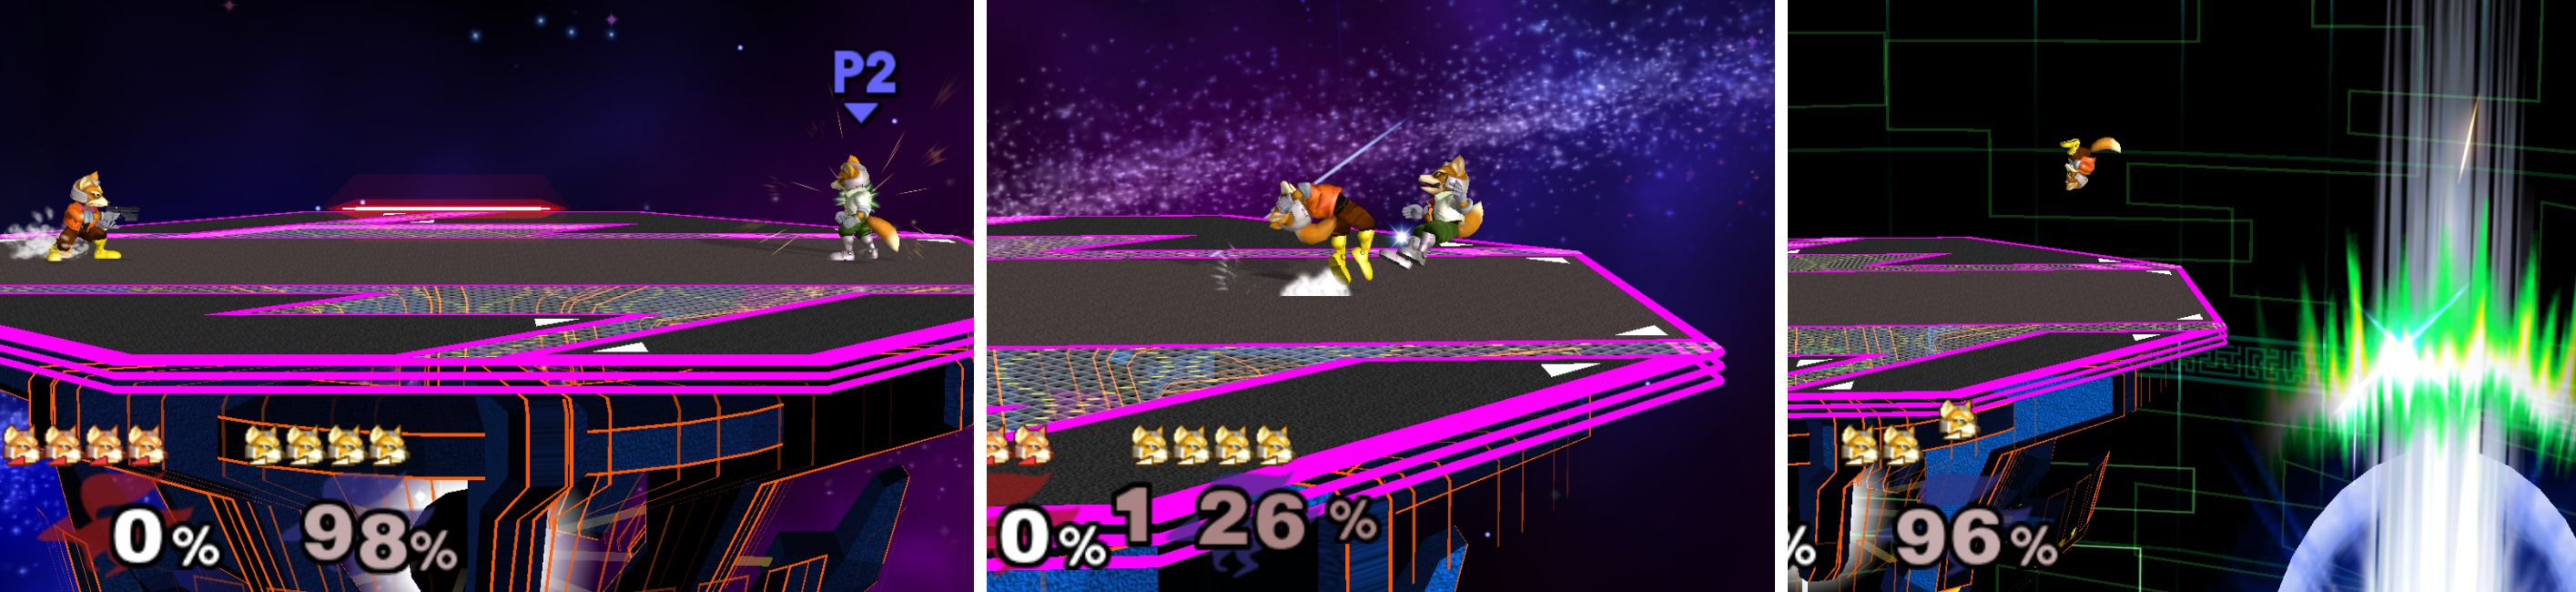
\includegraphics[width=\linewidth]{fig/hero.jpg}\\[8pt]
							{\small\badge{aILRL}{4}\,\textbf{\color{aILRL}imitation + RL}: up-throw, up-air, jab,
							up-smash, like a person}\\[4pt]
							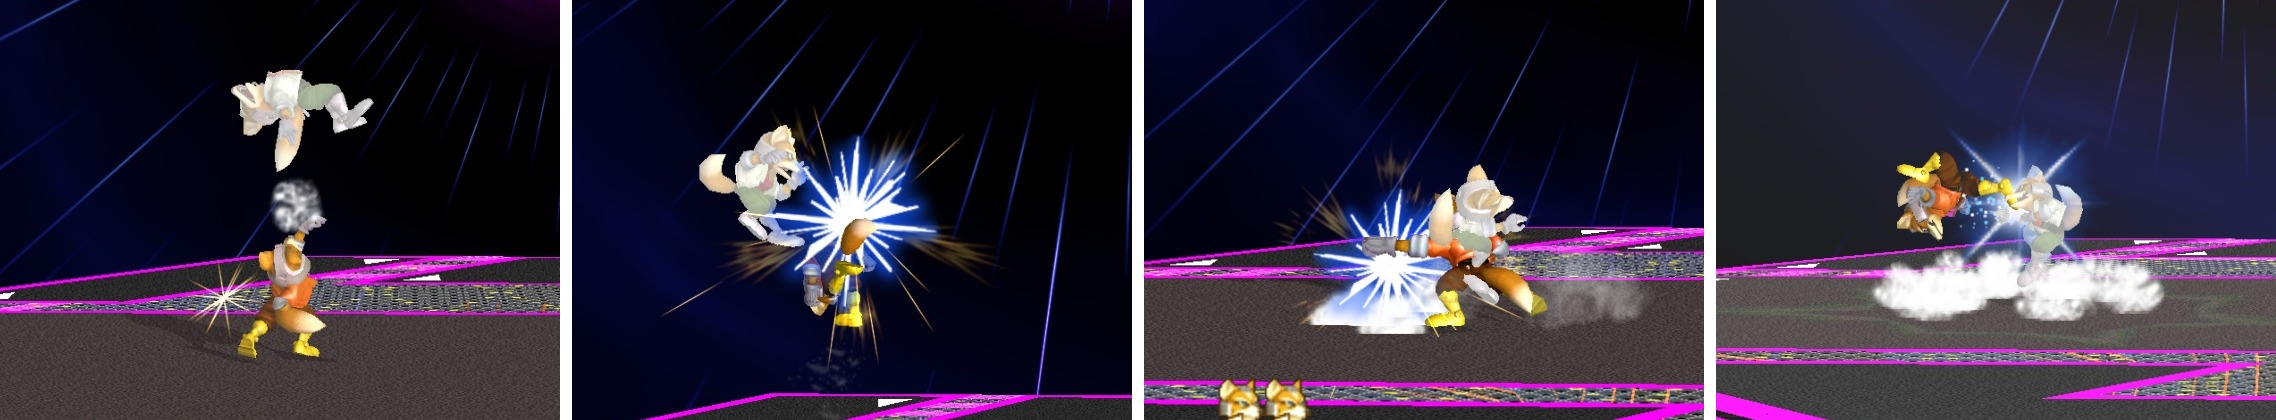
\includegraphics[width=\linewidth]{fig/kepiti_combo_strip.jpg}
							\caption{Against the level 9 CPU, captured from the emulator. Pure RL wins every game, but
							not the way people play.}
						\end{figure}
						\begin{itemize}
							\item \textbf{Melee}: 60 frames/s, frame-precise technique. Deep RL has beaten pros
							\cite{firoiu2017}, but by reacting faster than any human; our first PPO bots won by
							\textbf{exploiting} the game (spamming smash attacks, lasers, shields).
							\item We train one character, Fox, four ways and compare them on the same stage and rules.
						\end{itemize}
					\end{myblock}\vfill
					\begin{myblock}{Hypothesis}
						\begin{center}
							\agentcard{aRL}{1}{Pure RL}{PPO from scratch, sees the game instantly}
								{strongest against scripted opponents}{superhuman reactions, exploits the reward}\hfill
							\agentcard{aDelay}{2}{RL + reaction delay}{the same, but sees the game 200\,ms late}
								{fair: a human reaction time}{much harder to learn, weaker}\\[10pt]
							\agentcard{aIL}{3}{Imitation}{copies 111k games of strong players}
								{human technique: wavedash, L-cancel, shine}{copies mistakes, never tries to win}\hfill
							\agentcard{aILRL}{4}{Imitation + RL}{3, then RL on a leash to the human policy}{human style and wins}{depends on the human data}
						\end{center}
						\vspace{6pt}
						{\bfseries H:} with a human reaction time, \badge{aILRL}{4} beats \badge{aDelay}{2}, and pure RL
						\badge{aRL}{1} only avoids spam with heavy reward shaping.
					\end{myblock}\vfill
					\begin{myblock}{Problem formulation}
						\begin{itemize}
							\item \textbf{Observe} both players' state from memory (no pixels): position, speed,
							damage, stocks, action state, character.
							\item \textbf{Act}: \badge{aRL}{1}\badge{aDelay}{2} 31 stick + button macros, one every 2 frames;
							\badge{aIL}{3}\badge{aILRL}{4} a full controller every frame ($\approx 69$k choices).
							\item \textbf{React}: how late each agent sees the game \cite{firoiu2018}:
						\end{itemize}
						\begin{center}
							\begin{tikzpicture}[x=0.86cm, y=1cm]
								\fill[ETH3!10] (12,-0.55) rectangle (15,0.55);
								\node[font=\scriptsize, text=ETH3!80, above] at (13.5,0.55) {humans 200--250\,ms};
								\draw[line width=2pt, ETH3!60] (0,0) -- (19.5,0);
								\foreach \i in {0,...,19} {\draw[line width=1.5pt, ETH3!60] (\i,-0.18) -- (\i,0.18);}
								\node[below=3pt, font=\scriptsize] at (0,-0.2) {see frame $t$};
								\foreach \f/\c/\n/\l in {2/aRL/1/{$\le$ 2 frames}, 12/aDelay/2/{12 frames = 200\,ms},
									18/aILRL/{3,4}/{18 frames = 300\,ms}} {
									\fill[\c] (\f,0) circle (0.3);
									\node[below=10pt, font=\scriptsize, text=\c, align=center] at (\f,-0.2)
										{\bfseries \n\\ \l};
								}
							\end{tikzpicture}
						\end{center}
					\end{myblock}\vfill
					\begin{myblock}{The four agents}
						\begin{center}
							\begin{minipage}{0.24\linewidth}\centering
								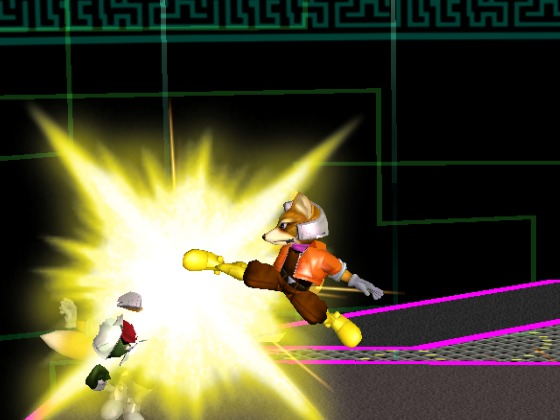
\includegraphics[width=\linewidth]{fig/agent_rl.jpg}\\[2pt]\badge{aRL}{1}\end{minipage}\hfill
							\begin{minipage}{0.24\linewidth}\centering
								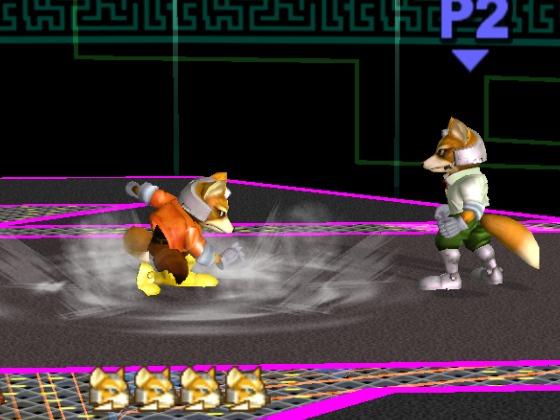
\includegraphics[width=\linewidth]{fig/agent_delay.jpg}\\[2pt]\badge{aDelay}{2}\end{minipage}\hfill
							\begin{minipage}{0.24\linewidth}\centering
								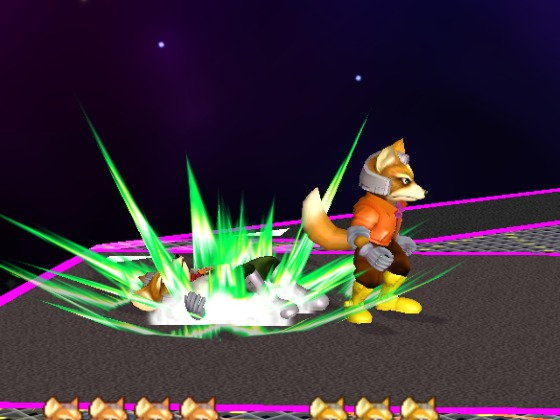
\includegraphics[width=\linewidth]{fig/agent_il.jpg}\\[2pt]\badge{aIL}{3}\end{minipage}\hfill
							\begin{minipage}{0.24\linewidth}\centering
								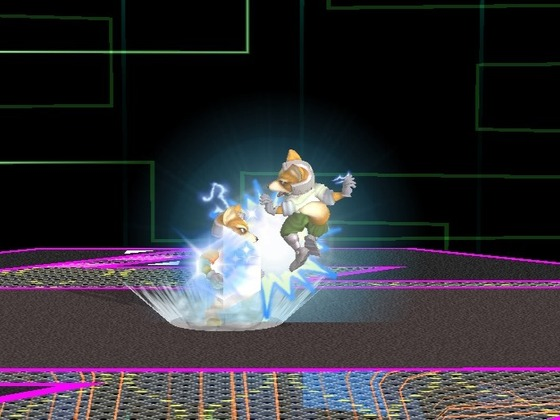
\includegraphics[width=\linewidth]{fig/agent_ilrl.jpg}\\[2pt]\badge{aILRL}{4}\end{minipage}
						\end{center}
						\vspace{4pt}
						{\footnotesize
						\begin{tabularx}{\linewidth}{@{}l>{\raggedright\arraybackslash}X>{\raggedright\arraybackslash}X@{}}
							\toprule
							& \textbf{Policy network} & \textbf{Learns from} \\
							\midrule
							\badge{aRL}{1} & MLP actor + critic, $2 \times 256$ ReLU, 0.6\,M parameters
								& CPU curriculum level 1 $\rightarrow$ 9 \cite{curriculum}, then a league of frozen
								past agents \cite{alphastar} \\
							\badge{aDelay}{2} & the same, fed the state of 12 frames ago & starts from
								\badge{aRL}{1}\,, then the same league \\
							\badge{aIL}{3} & $3 \times$ (LSTM \cite{lstm} + MLP), width 512, 9.9\,M parameters
								\cite{slippiai} & 111k ranked games of master / diamond Fox players \cite{dataset} \\
							\badge{aILRL}{4} & the same & starts from \badge{aIL}{3}\,, then self-play, a Ganondorf
								bot and the level 9 CPU \\
							\bottomrule
						\end{tabularx}}
					\end{myblock}\vfill
		}\end{minipage}\end{beamercolorbox}
	\end{column}
	\begin{column}{.5\textwidth}
		\begin{beamercolorbox}[center]{postercolumn}
			\begin{minipage}{.98\textwidth} % tweaks the width, makes a new \textwidth
				\parbox[t][\columnheight]{\textwidth}{
					\begin{myblock}{Method: reinforcement learning \badge{aRL}{1}\,\badge{aDelay}{2}}
						PPO \cite{ppo,sb3} with GAE \cite{gae} ($\gamma = 0.995$, $\lambda = 0.95$, $\epsilon = 0.2$),
						8 headless emulators in parallel \cite{libmelee,slippi}:
						\begin{equation*}
							\mathcal{L}(\theta) = -\,\mathbb{E}_t\Big[\min\big(\rho_t \hat{A}_t,\,
							\mathrm{clip}(\rho_t, 1 \pm \epsilon)\,\hat{A}_t\big)\Big]
							\qquad \rho_t = \frac{\pi_\theta(a_t \mid o_t)}{\pi_{\text{old}}(a_t \mid o_t)}
						\end{equation*}
						\textbf{Shaped reward} \cite{shaping}, per frame: knockouts first, combos pay, spam costs:
						\begin{equation*}
							\begin{aligned}
							r_t = {}& 2\,\big(\Delta \text{KO}_{\text{opp}} - \Delta \text{KO}_{\text{own}}\big)
							+ 0.003\,\big(\Delta\%_{\text{opp}} - \Delta\%_{\text{own}}\big)\\
							&+ r^{\text{combo}}_t - r^{\text{whiff}}_t - r^{\text{spam}}_t - r^{\text{camp}}_t
							\end{aligned}
						\end{equation*}
						\begin{itemize}
							\item $r^{\text{combo}}$: $0.1\,k$ for the $k$-th hit of a listed combo; $r^{\text{whiff}}$:
							0.03 per missed attack, 0.2 per missed smash.
							\item $r^{\text{spam}}$: the $n$-th repeat of a smash, move or dodge costs
							$\min(2,\, b\, 2^{\,n-2})$, doubling up to one knockout. \badge{aDelay}{2} acts on $o_{t-12}$.
						\end{itemize}
					\end{myblock}\vfill
					\begin{myblock}{Method: learning from humans \badge{aIL}{3}\,\badge{aILRL}{4}}
						\textbf{Behaviour cloning} \badge{aIL}{3}: predict the human's controller 18 frames ahead
						\cite{slippiai}:
						\begin{equation*}
							\mathcal{L}_{\text{BC}}(\theta) = -\sum_t \sum_{k=1}^{4}
							\log \pi_\theta\big(a^{(k)}_{t+18} \,\big|\, h_{t},\, a^{(<k)}_{t+18}\big)
						\end{equation*}
						\textbf{RL on a leash} \badge{aILRL}{4}: the PPO loss above plus a KL penalty to the frozen
						imitation policy \cite{seqtutor,alphastar},
						$\;\mathcal{L}(\theta) = \mathcal{L}_{\text{PPO}}(\theta)
						+ \beta\, \mathbb{E}_t\big[\KL\big(\pi_\theta \,\|\, \pi_{\text{BC}}\big)(h_t)\big]$,
						$\beta = 0.5$, $\gamma = 0.997$; reward: stocks and damage.
					\end{myblock}\vfill
					\begin{myblock}{Training (preliminary)}
						\begin{center}
							\stattile{aRL}{$\approx$\,91\,h}{pure RL}{90\,M steps, 8 games}\hfill
							\stattile{aDelay}{+12\,h}{RL + delay}{12\,M steps, from \badge{aRL}{1}}\hfill
							\stattile{aIL}{18\,h}{imitation}{1.24\,B frames, 1 GPU}\hfill
							\stattile{aILRL}{+3\,h}{imitation + RL}{10 games, from \badge{aIL}{3}}
						\end{center}
						\vspace{6pt}
						\begin{center}
							\placeholder{0.97\linewidth}{3.5cm}{\textbf{Training curves of the four agents} (final runs
							still going)\\[6pt] win rate against the level 9 CPU, stock lead and share of attacks
							that miss, against training time}
						\end{center}
						\begin{itemize}
							\item So far: \badge{aRL}{1} wins 100\% against the level 9 CPU; the spam penalties cut
							smash-attack spam from $\sim$24 to $\sim$4 per game. With the 200\,ms delay, learning from
							scratch stalled at CPU level 4--5, so \badge{aDelay}{2} starts from \badge{aRL}{1}.
						\end{itemize}
					\end{myblock}\vfill
					\begin{myblock}{Results: final tournament}
						\begin{columns}[T]
							\begin{column}{0.47\textwidth}
								{\footnotesize\centering
								\begin{tabularx}{\linewidth}{@{}l*{6}{Z}@{}}
									\toprule
									& \badge{aRL}{1} & \badge{aDelay}{2} & \badge{aIL}{3} & \badge{aILRL}{4} & CPU & Gan. \\
									\midrule
									\badge{aRL}{1} & -- & ? & ? & ? & ? & ? \\
									\badge{aDelay}{2} & ? & -- & ? & ? & ? & ? \\
									\badge{aIL}{3} & ? & ? & -- & ? & ? & ? \\
									\badge{aILRL}{4} & ? & ? & ? & -- & ? & ? \\
									\bottomrule
								\end{tabularx}\par}
								\vspace{4pt}
								{\scriptsize Win rate of the row agent. Final Destination, 4 stocks, ? games per pair;
								CPU: level 9 Fox; Gan.: the Ganondorf PPO bot.}
							\end{column}
							\begin{column}{0.5\textwidth}
								\placeholder{\linewidth}{4.3cm}{\textbf{Tournament figure}\\[4pt] win rates and
								play style (attacks, combos, spam per minute) of the four agents}
							\end{column}
						\end{columns}
					\end{myblock}\vfill
					\begin{myblock}{Conclusion}
						\begin{itemize}
							\item \emph{(after the tournament)} which recipe wins with a human reaction time, at what cost
							in style. Next: more stages, games against people.
						\end{itemize}
					\end{myblock}\vfill
					\begin{myblock}{References}
						\tiny
						\begin{multicols}{3}
							\bibliographystyle{abbrv}
							\bibliography{./bib}
						\end{multicols}
					\end{myblock}\vfill
		}\end{minipage}\end{beamercolorbox}
	\end{column}
\end{columns}
\end{frame}
\end{document}
